The only supernova neutrinos detected to date was the SN1987A, from a supernova that happened at the Large Magellanic Cloud. A small amount of electron neutrinos from the event were observed at Kamiokande-II ($12 \nu_e$s), IMB ($8 \nu_e$s), and Baksan ($5 \nu_e$s). Despite the small dataset, a rich amount of analysis was published using the data, \cite{Kamiokande-II-PRL, Kamiokande-II-PRD, IMB, Baksan}. 
 On the occasion of a core-collapse supernova in our galaxy, measuring the flux of neutrinos and antineutrinos from all flavors will significantly enlighten the fields of astrophysics and neutrino physics. Therefore, one of DUNE's goals is to be prepared for such an event, as it is the most potent detector to measure the electron neutrinos signal from a supernova, \cite{dune_SAND}.
 In this chapter, I will explain the basics of supernovas and the neutrinos produced at them, why DUNE is particularly suitable to measure those neutrinos, and how using muos that decay at rest ($\mu$DARs) at the NuMI beam and interact in the MicroBooNE detector can help us improve neutrino-nucleus theoretical models and MeV-scale detection techniques in LArTPCs, which will be essential to accomplish the supernova detection in DUNE. 

\section{Core-Collapse Supernova Neutrino Detection in DUNE}
\subsubsection{Supernovas}
Supernova is the name given to the explosive chain of events that happens during the death of some stars. Mainly, core-collapse supernovas produce a massive number of neutrinos and antineutrinos whose spectrum, if measured, can inform the characteristics of the explosion. 
At the end of the life of a star that has $8-40$ solar masses, its body is made of concentric shells that were formed at each of its previous burning phases, them being: hydrogen, helium, carbon, neon, oxygen, silicon, enveloping a core of nickel and iron. During its life, the stability of the star is a balance between the thermal pressure produced in the fusion process, which pulls everything in the outer direction, and its gravity pulling inward. When the mass of the iron core reaches $1.4$ solar masses, the pressure is not enough to balance the gravity, and the core starts to be compressed by the outer layers. Temperature and density in the core rise and the reaction

\begin{equation}
    e^{-} + p \longrightarrow n + \nu_e
\end{equation}

starts to happen more frequently, causing the pressure from electrons to lower even more and the star to collapse more rapidly. At the latest stages of the collapse, the density is such that even neutrinos get trapped in the core. Eventually, the pressure created by the nucleons degeneracy interrupts the collapse. The sudden stop of the collapse in the core causes a shock wave through the outer layers, and the star explodes. At the early stage of the shock wave, the density lowers, and the neutrinos manage to escape, creating an intense few-millisecond pulse called neutronization burst. 
After the neutronization burst, outer layers of the star still falling innard manage to stall the shock wave briefly. This stage is called the accretion phase. We still don't understand why the shock wave regains energy enough to proceed. One hypothesis is that neutrino reactions produce sufficient heat for the thermal pressure to give continuity to the explosion. 
Next, in the cooling phase, the star's energy is given away in many different processes that create neutrinos and antineutrinos of various flavors. A few of them are:

\begin{align}
    & \text{{\color{gray} electron pair annihilation:}}
    && e^{-} + e^{+} \longrightarrow \nu + \bar{\nu}, \\
    & \text{{\color{gray}electron-electron neutrino bremsstrahlung:}}
    && e^{\pm} + e^{\pm} \longrightarrow e^{\pm} + e^{\pm} + \nu + \bar{\nu} \\
    & \text{{\color{gray}electron-nucleon neutrino bremsstrahlung:}}
    && e^{\pm} + N \longrightarrow e^{\pm} + N + \nu + \bar{\nu} \\
    & \text{{\color{gray}photoannihilation:}}
    && \gamma + e^{\pm} \longrightarrow e^{\pm} + N + \nu + \bar{\nu} \\
    & \text{{\color{gray}nuclear de-excitation by neutrino pair production:}} 
    && ^{Z}_{A}X^{*} \longrightarrow ^{Z}_{A}X + \nu + \bar{\nu}
\end{align}

Given the wide variety of processes, measuring the flux of neutrinos and antineutrinos from all flavors is fundamental to help us better understand aspects of the supernova and what role the processes during the explosion play in its development, \cite{Gardiner_thesis}. 

\subsubsection{Supernova detection in DUNE}

We have in operation or planned for the future a number of large detectors that would be able to detect signals from a core-collapse supernova that happens in our galaxy. The active material of those detectors is either water Cherenkov or hydrocarbon scintillator, making them mainly sensitive to electron antineutrinos via inverse beta decay (the reaction in equation \ref{inverse_beta_decay_eq}). 
Therefore, relying solely on those detectors would preclude the measurement of the supernova electron neutrino flux, which is the most significant component produced during the supernova's neutronization phase. 

Luckily, DUNE's active material is liquid argon, which is mainly sensitive to eletron neutrinos, via charged current scattering in $^{40}$Ar, as in:

\begin{equation}
    \nu_e + ^{40}Ar \longrightarrow ^{40}K + e^{-}
    \label{nu_scatter_eq}
\end{equation}
 
An example of a contribution to neutrino physics that a supernova neutrino detection could make in DUNE is to shine light into the mass hierarchy puzzle. Figure \ref{dune_supernova} shows how the time distribution of the incoming flux of the neutrinos of a $10$ kpc supernova in DUNE could depend on the mass hierarchy. In the case of inverted hierarchy, we should see an early excess of events from the neutronization phase, whether, in the case of normal hierarchy, we should see the absence of such events. The results from figure \ref{dune_supernova} are made assuming a model describer in reference \cite{dune_supernova_model}, but those results are assumed to be fairly model-independent \cite{kate_scholberg}. 

\begin{figure}[h!]
    \centering
    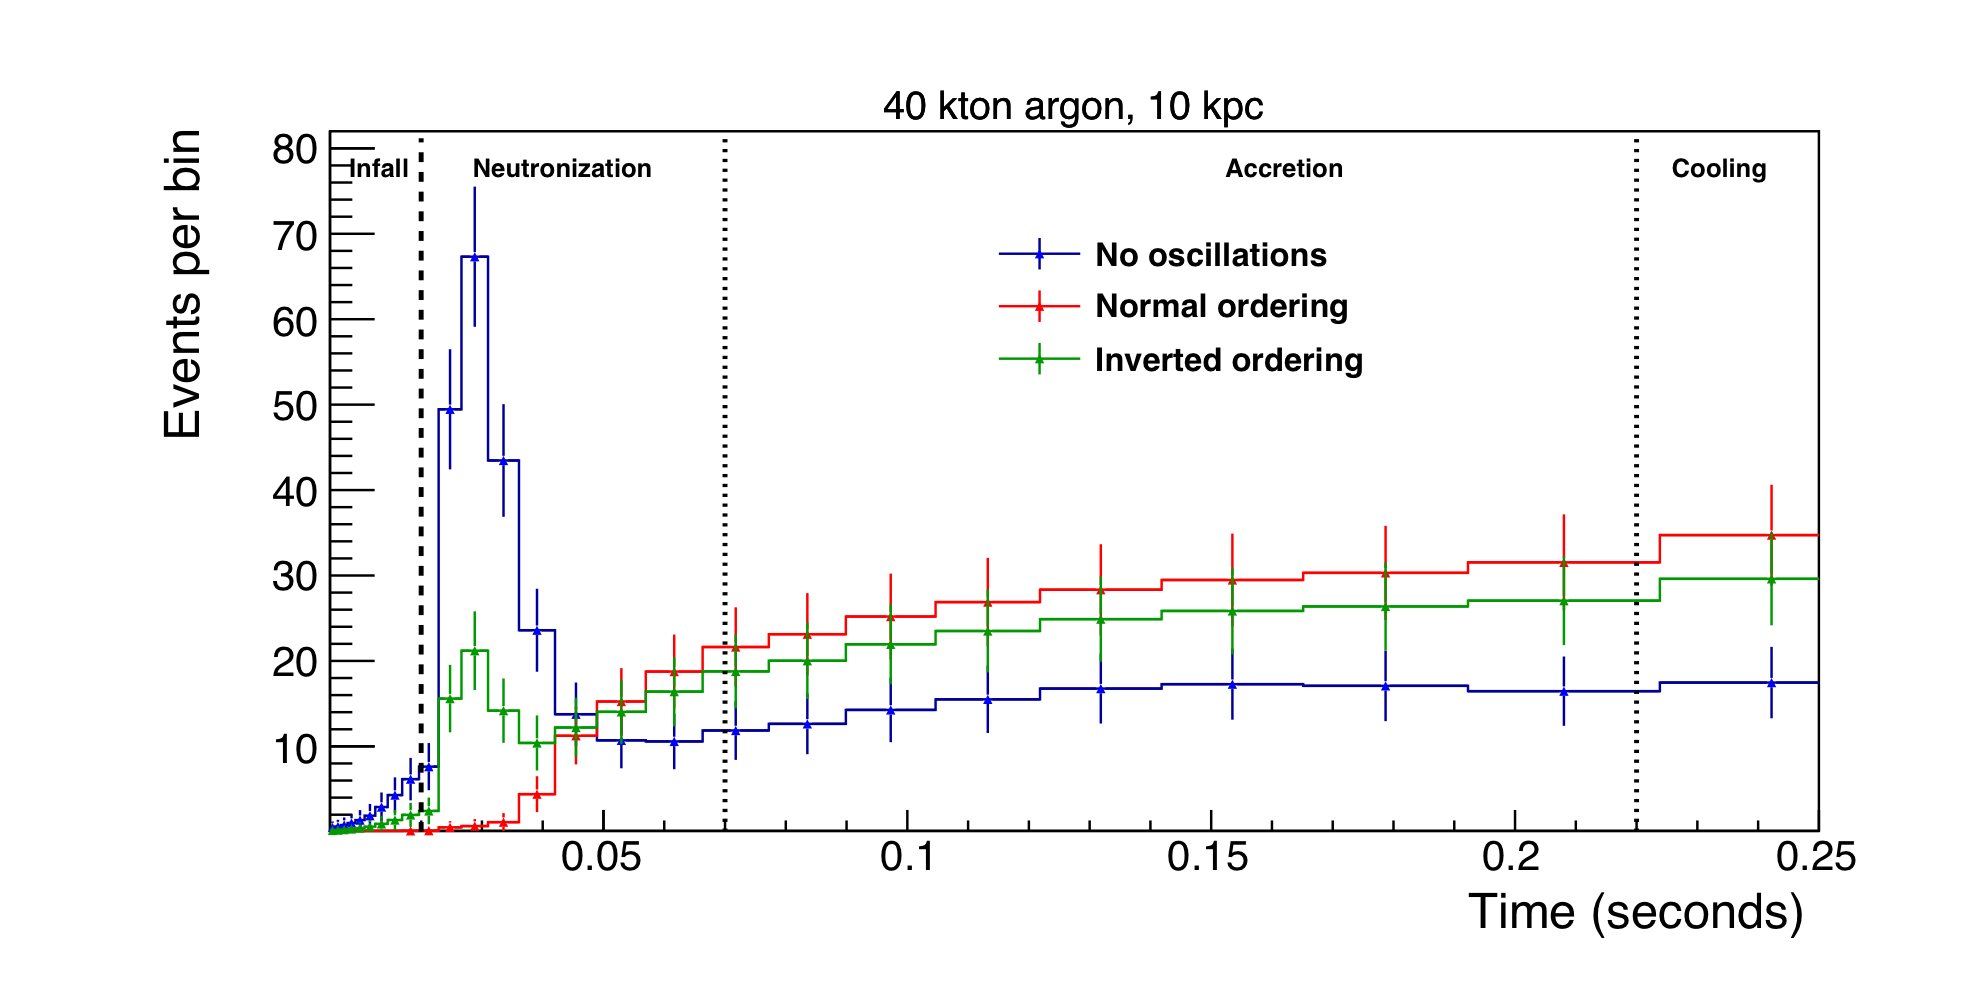
\includegraphics[width=150mm]{Figures/dune_supernova.jpeg}
    \caption[Predicted event time distribution for the detection of supernova neutrinos in a DUNE-like $40$ kt LArTPC]{{\textbf{Predicted event time distribution for the detection of supernova neutrinos in a DUNE-like 40 kt LArTPC}}\\ Predicted event time distribution for the detection of a $10$ kpc supernova neutrinos in a DUNE-like 40 kt LArTPC for each of the supernova stages. The blue curve assumes no oscillations, the green and the red curves assume oscillations for inverted and normal mass hierarchy, respectively \cite{kate_scholberg}.}Furthermore, being able to measure the flux of both neutrinos and antineutrinos is fundamental to further understanding exotic supernova processes \cite{Friedland}.
    \label{dune_supernova}
\end{figure}

Furthermore, being able to measure the flux of both neutrinos and antineutrinos is fundamental to further understanding exotic supernova processes \cite{Friedland}. 

\section{$\mu$ Decay At Rest $\nu_e$ Charged Current interactions in MicroBooNE}

\subsection{$\mu$ Decay At Rest in MicroBooNE}
As promising as the DUNE supernova neutrino program is, we currently lack an understanding of the MeV-scale neutrinos and LAr nucleus interactions, LArTPC reconstruction capabilities, and event identification at this energy range. 

As mentioned before, MicroBooNE is exposed to the BNB and NuMI beamlines. When on FHC mode, both beamlines produce a copious amount of antimuons that will, when decaying at rest, produce a muon antineutrino, an electron neutrino, and a positron, as shown in equation \ref{mudar_decay_eq}. The energy spectrum of the electron neutrinos from this decay is well-known and can be seen in picture \ref{mudar_nue_energy}. In figures \ref{numi_nue_flux} and \ref{numi_nu_flux} you can see the NuMI flux prediction of $\nu_e$s in MicroBoone by parents and the NuMI flux prediction in MicroBooNE of all neutrinos, respectively. 

\begin{equation}
	\mu^{+} \longrightarrow e^{+} + \nu_e + \bar{\nu}_{\mu}
    \label{mudar_decay_eq}
\end{equation}

\begin{figure}[h!]
    \centering
    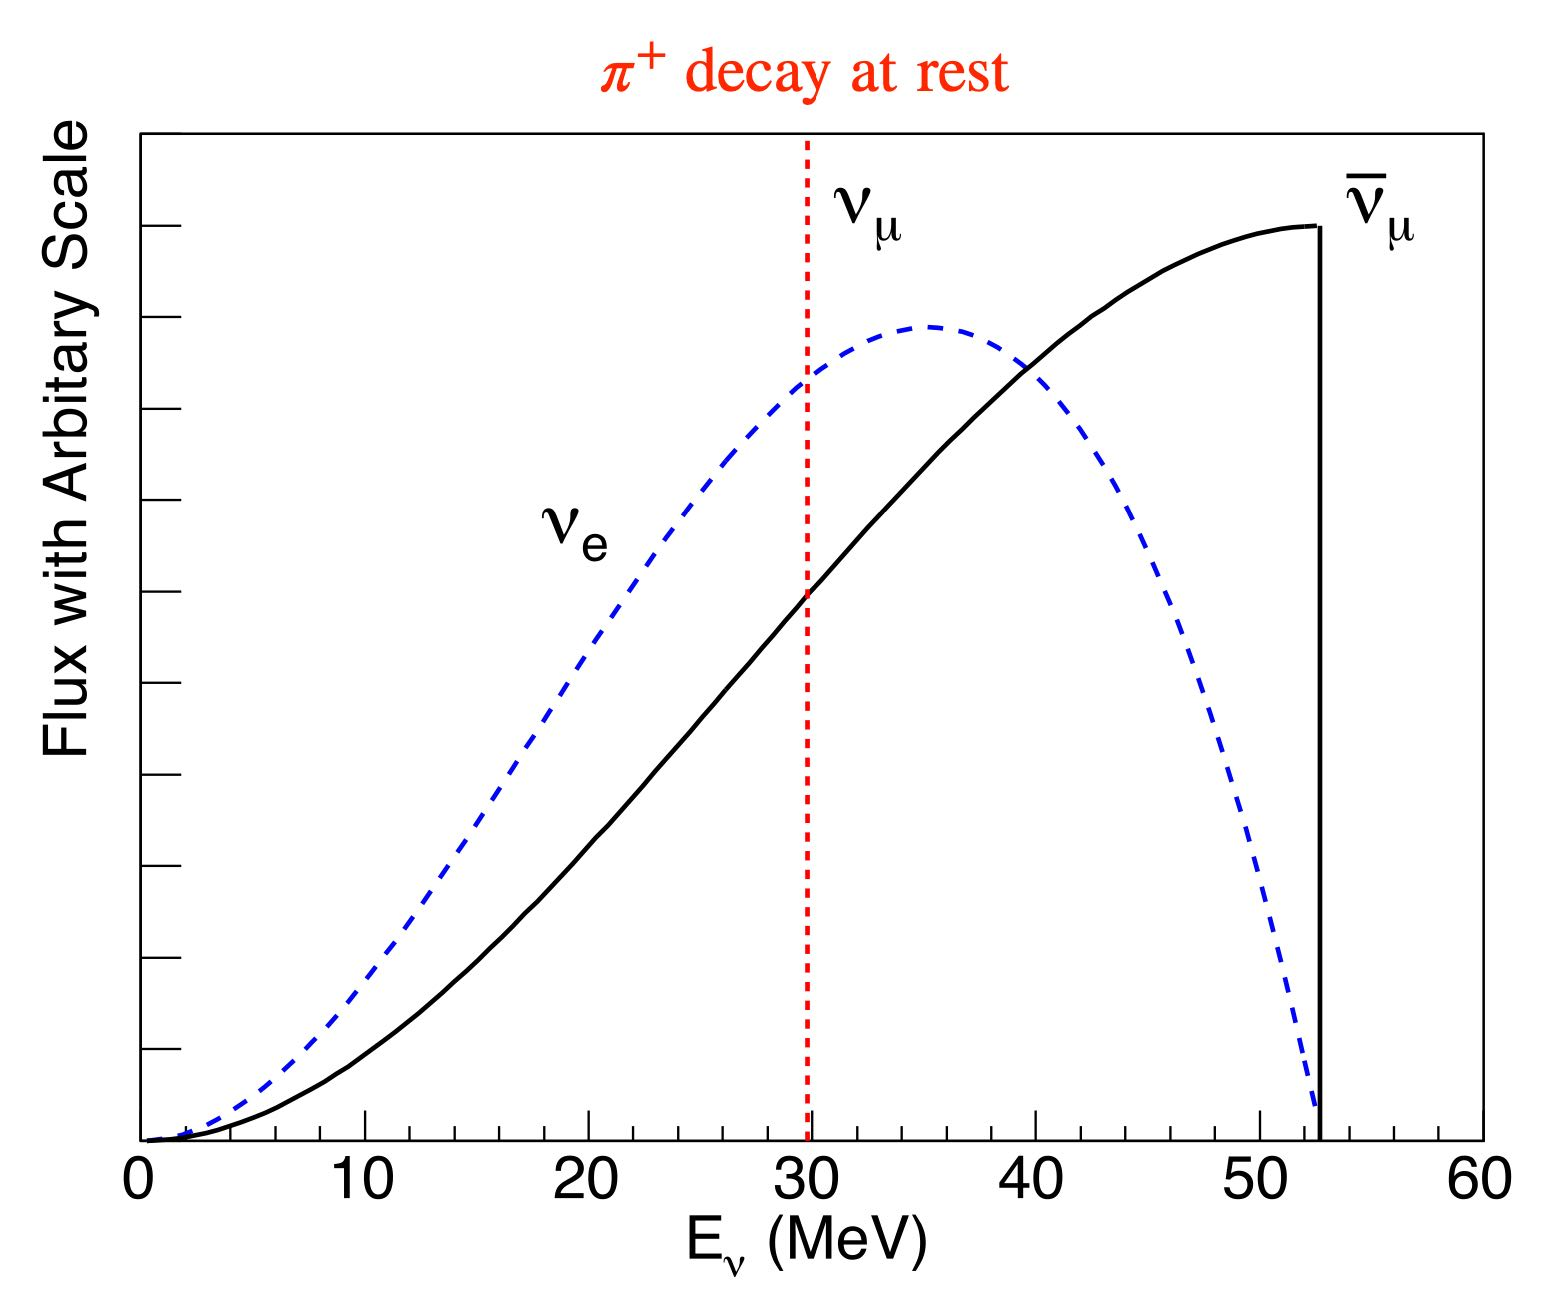
\includegraphics[width=110mm]{Figures/mudar_nue_energy.jpg}
    \caption[Neutrino spectra of pion and muon decay at rest]{{\textbf{Neutrino spectra of pion and muon decay at rest}}\\ The red line is the energy of muon neutrinos from pion decay at rest, which is well-defined. The blue and the black lines refer to the energy spectrum of electron neutrinos and muon antineutrinos from positive muon decay at rest, respectively \cite{Yang2012}.}
    \label{mudar_nue_energy}
\end{figure}

Due to the nature of the decay, the electron neutrino will have kinetic energy $0 \leqslant KE_{\nu_e} \leqslant 52.8$ MeV, which overlaps nicely with the energy range of the supernova electron neutrinos we aim to detect in DUNE!

\begin{figure}[h!]
    \centering
    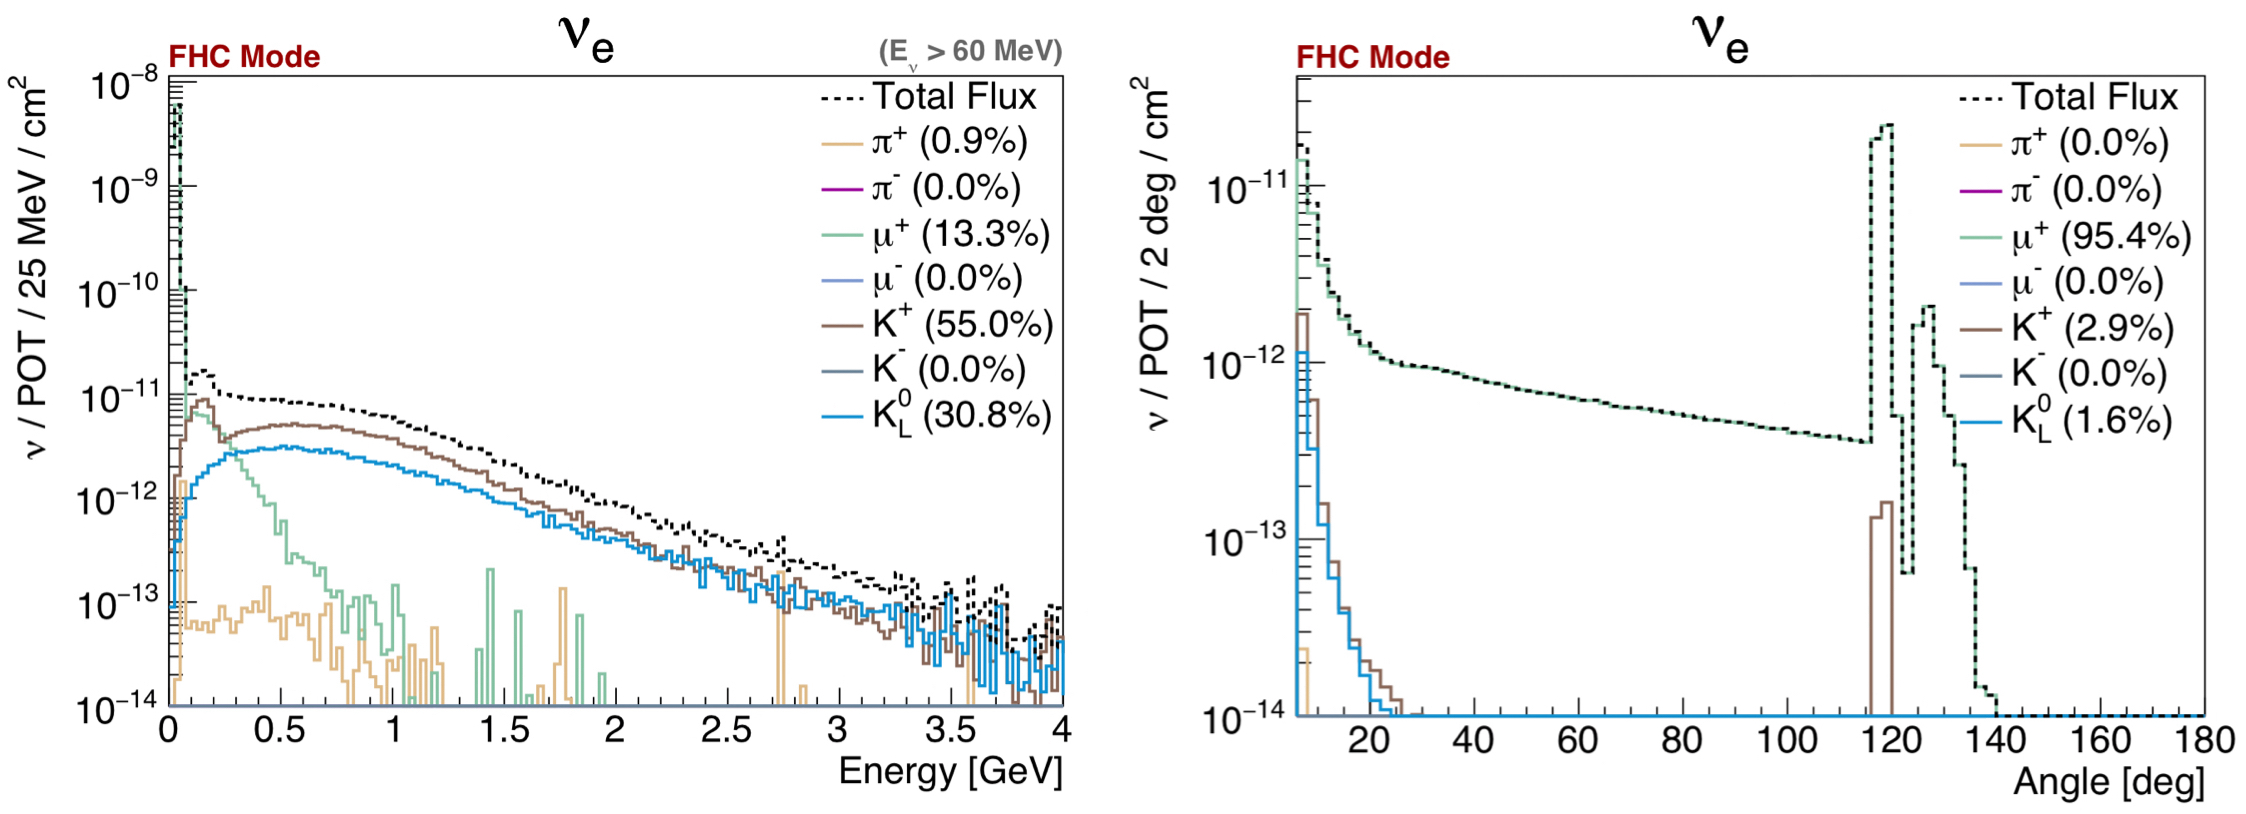
\includegraphics[width=180mm]{Figures/numi_nue_flux.jpeg}
    \caption[NumI $\nu_e$ flux in MicroBooNE]{{\textbf{NumI $\nu_e$ flux in MicroBooNE}}\\ On the right, the FHC $\nu_e$ neutrino flux at MicroBooNE from NuMI broken down by parent. Although a 60 MeV threshold is included in the percentages, the absolute value clearly shows the dominance of muon decays. On the left, the FHC neutrino flux is broken down by parent for each neutrino flavor. The percentages shown do not include an integration threshold on the angle. Decays from pions and muons dominate the majority of the flux across all angles \cite{krish_phd}.}
    \label{numi_nue_flux}
\end{figure}

\begin{figure}[h!]
    \centering
    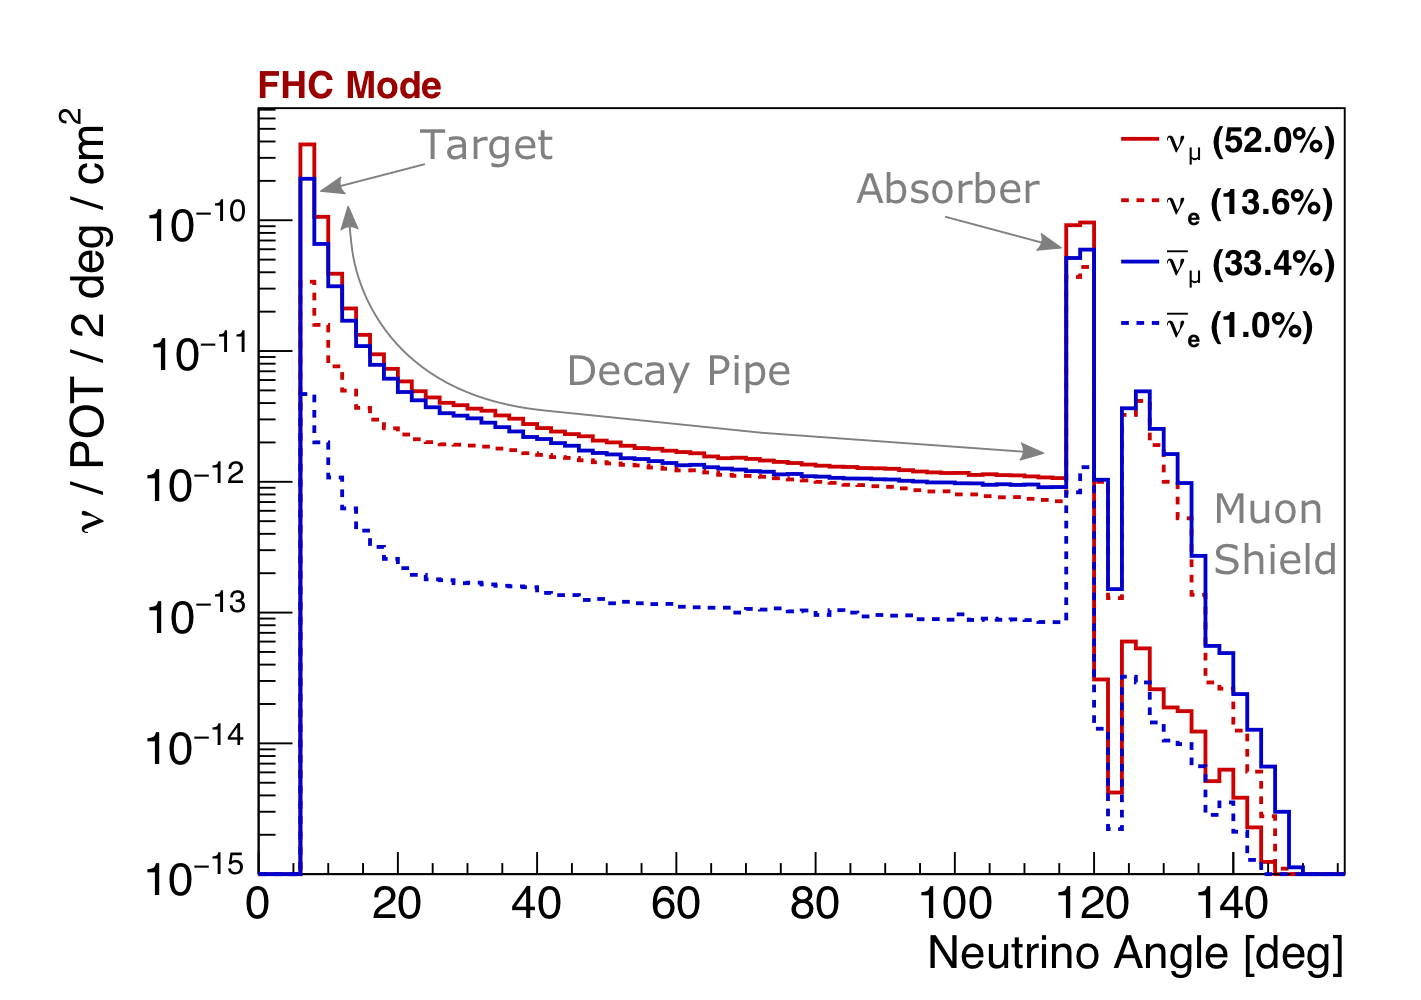
\includegraphics[width=130mm]{Figures/numi_nu_flux.jpeg}
    \caption[NumI $\nu$ flux in MicroBooNE]{{\textbf{NumI $\nu$ flux in MicroBooNE}}\\ The flux prediction for all neutrino flavours in the FHC mode in neutrino angle. No integration threshold is applied in the percentages, and the electron neutrino flux percentage is boosted by muon decay at rest. The large angular spread in the flux is due to the positioning of MicroBooNE with respect to the NuMI beamline. The flux peaks at the target location and tails off further into the beamline. From angles above $20$ deg (midway into the decay pipe), the flux remains flat up to the absorber, where there is a large peak in the flux spectrum $\approx 120$ deg. After this, the flux is attenuated rapidly going into the muon-shield $ \ge 120$ deg.\cite{krish_phd}.}
    \label{numi_nu_flux}
\end{figure}
\newpage

\subsection{MeV-scale $\nu_e$-LAr Charged Current Interactions}

As explicitly shown in the \ref{nu_scatter_eq}, when MeV-scale neutrinos scatter in $^{40}$Ar, we have as product a $^{40}\textrm{K}^{*}$ and a $e^{-}$. From now on, I will refer to this electron as the ``main" electron of the signal. The energy of the incoming neutrino can be reconstructed as:

\begin{equation}
    E_{\nu} = E_e + \Delta_{final-initial} + T_{recoil} 
    \label{E_mudar_nu}
\end{equation}

where $E_e$ is the total energy of the outcoming electron and $T_{recoil}$ is the kinetic energy of the recoiling nucleon (which is negligible). As for $\Delta_{final-initial}$: 

 \begin{equation}
    \Delta_{final-initial} \equiv m_{final} - m_{initial}  
    \label{delta_fi}
\end{equation}

where $m_initial$ is the mass of the initial $^{40}$Ar nucleus, and $m_{final}$ is the mass state of the $^{40}\textrm{K}^{*}$ nucleus. The potassium nucleus can be at different excited states, depending on the event. Therefore, $m_{final}$ can be further described as:

\begin{equation}
    m_{final} = m_{final, g.s.} + E_x
    \label{mfinal}
\end{equation}

where $m_{final, g.s.}$ is the ground-state mass of a $^40$K nucleus and $E_x$ is the excitation energy. To reconstruct the total energy from the incoming neutrino, we need to look into the products from the de-excitation of the excited potassium nucleus, which are most commonly photons. Those photons can be indirectly measured in LArTPCs as they scatter on Ar atomic electrons, and the value of $\Delta_{final-initial}$ is given by:

\begin{equation}
    \Delta_{final-initial} = m_{g.s. \rightarrow g.s.} + \sum_{j}E_{\gamma, j}   
    \label{delta_fi_2}
\end{equation}

where $E_{\gamma,j}$ is the energy of each of the photons emitted and $m_{g.s. \rightarrow g.s.}$ is the mass difference between the ground state of the $^{40}$K nucleus and the ground state of the $^{40}$Ar nucleus, which is $1.5044$ MeV. 
It is also possible, although less likely, to have the excitation energy of the $^{40}$K high enough such that the de-excitation proceeds with the emission of a nucleon. A few of these channels still leave the daughter nucleus in an excited state, and there is an additional $\gamma$-ray or nucleon emission. This cascade continues until the daughter nucleus reaches the ground state. A diagram representing the different de-excitation channels can be seen in figure \ref{40K_deexcite}

\begin{figure}[h!]
    \centering
    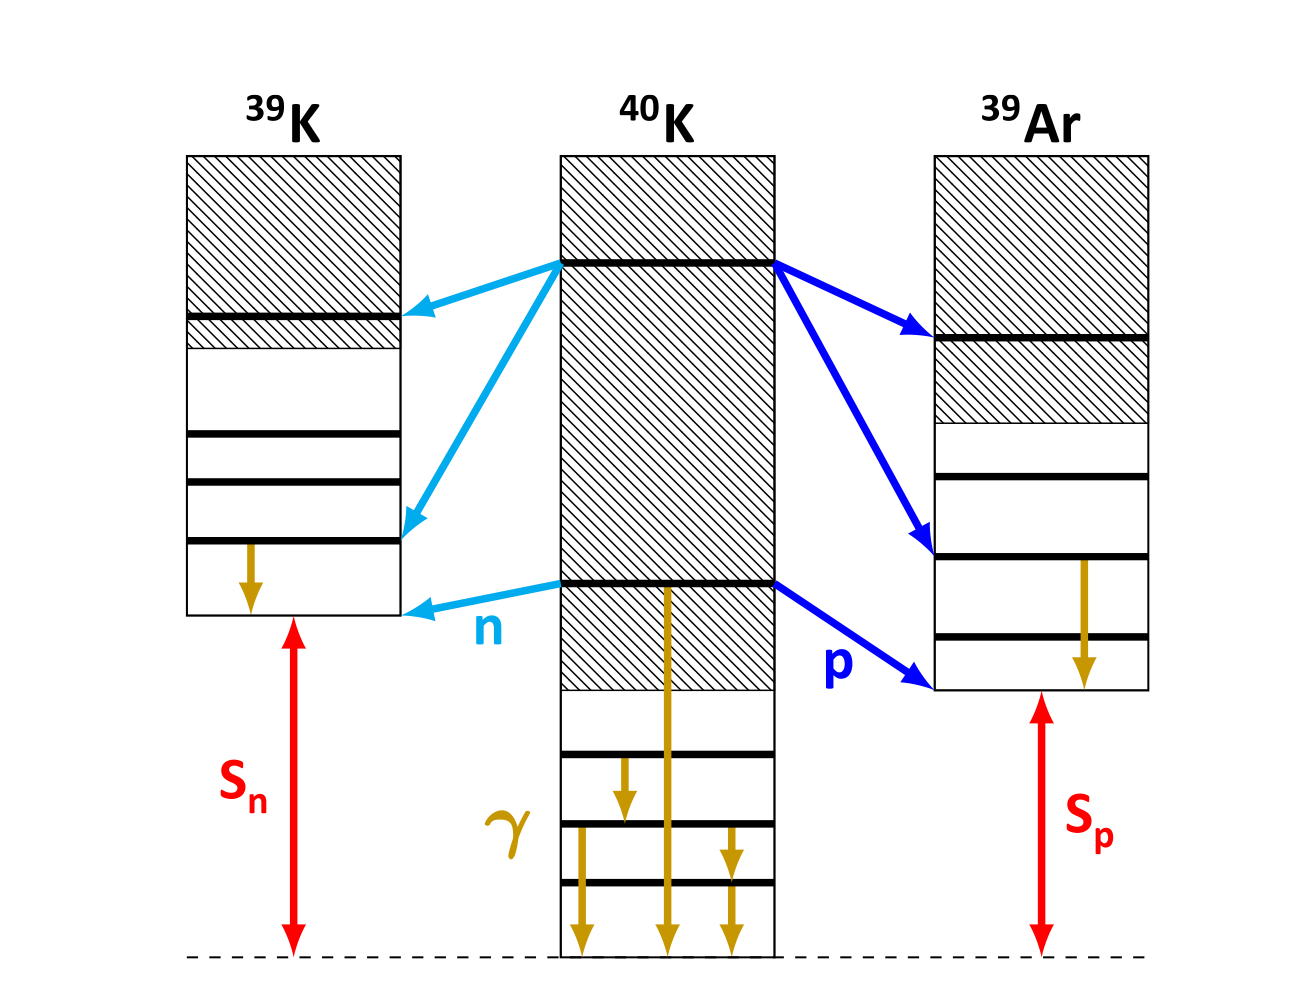
\includegraphics[width=135mm]{Figures/40K_deexcitation.jpeg}
    \caption[De-excitation channels from an excited $^{40}$K nucleus, product of a CC MeV-scale $\nu_e$-LAr scattering]{{\textbf{De-excitation channels from an excited $^{40}$K nucleus, product of a CC MeV-scale $\nu_e$-LAr scattering}}\\  The excited $^{40}$K nucleus can reach its ground state by emitting $\gamma$-ray(s) (middle diagram), a neutron (diagram on the left), or a proton (diagram on the right). In case the emission of a nucleon still leaves the daughter nucleus in an excited state, more photons are emitted until the ground state is reached \cite{Gardiner_thesis}.}
    \label{40K_deexcite}
\end{figure}

The complexity of nuclear structures and the possible final state topologies for those interactions add challenges to the proper energy reconstruction of the supernova neutrino events. Therefore, it is fundamental that we take the opportunity presented by $\mu$DAR $\nu_e$s in MicroBooNE to study these interactions to improve our techniques. 


\section{Simulation of $\mu$DAR Events in MicroBooNE}

To properly evaluate the $\mu$DAR events in MicroBooNE, we count with a chain of different simulation software to mimic the particle production and interactions at each step of the way, from the early stages of the beamline to MicroBooNE's detector response. 
To explicitly name the sequence, we start at the NuMI beam flux simulation, to the Generates Events for Neutrino Interaction Experiments (GENIE) Generator, and to the Model of Argon Reaction Low Energy Yields (MARLEY) Generator, back to the GENIE again, then to Geant4. All these softwares are integrated into a larger framework called the Liquid Argon Software (LArSoft). I will further go over each of these in this section. 

\subsection{Geant4}

 Geant4 \cite{g4} is a software toolkit that simulates the interaction of particles with matter. It can handle electromagnetic, decay, and hadronic physics interacting with complex geometries and variable EM fields. In MicroBooNE we use it during two steps of the simulation chain I described above: the NuMI beamline, and the propagation of the neutrino-LAr interaction products through LAr.

\subsection{NuMI Beam Simulation}

The NuMI beam flux simulation software has been continually developed by several experiments that use the NuMI beam, such as No$\nu$A, Main Injector Neutrino ExpeRiment to study $\nu-$A interactions (MINER$\nu$A) \cite{minerva}, and Main Injector Neutrino Oscillation Search (MINOS \cite{minos}. The software simulates the proton-target collision and its products, hadrons and muons that decay into neutrinos. MicroBooNE has two Geant4 packages that can used in the NuMI beamline simulation to handle different physics models to describe the hadron production: the g4numi\_flugg and the g4numi. In the g4numi\_flugg, FLUKA software framework is used to model the hadron production and Geant4 is used to handle the geometry of the beamline \cite{fluka}. In the g4numi, Geant4 is used for both model the hadron production and to handle the beamline geometry. In this thesis, we used the latter. 
The NuMI beam simulation also uses the Package to Predict the FluX (PPFX) to constrain the hadron production modeling and also propagate uncertainties through the beamline simulation \cite{ppfx}. Detailed description on the full NuMI beamline flux simulation can be found at \cite{krish}. 

Historically, both the NuMI beam and the BNB beam flux simulation had a minimum lower incoming neutrinos energy of $60$ MeV. This lower threshold was removed in the NuMI simulation, which, together with the higher flux of MeV-scale neutrinos, is why we opted to first perform this analysis using the NuMI beam instead of the BNB beam. 

\subsection{GENIE and MARLEY}
GENIE and MARLEY are software that falls in a specific category called ``neutrino event generators” and is specialized in neutrino-nucleus interactions. They are equipped with theoretical models of neutrino-nucleus interactions across a wide range of energies and targets. 
GENIE is the standard event generator used by MicroBooNE for physics analysis. In it, the target nucleus is modeled as a relativistic Fermi gas, i.e., non-interacting nucleons confined in a constant potential well. This makes it unfit to mimic the neutrino-nucleus interactions at the MeV-scale since the nuclear level structure is relevant for the characteristics of our final products, as described in the previous section. 
MARLEY, on the other hand, was designed to be especially capable of handling low-energy neutrino-nucleus interactions. It is based on a formalism to calculate low-energy neutrino-nucleus scattering called Walecka-Donnelly \cite{Walecka-Donnelly}. In it:
\begin{enumerate}
 \item the field gauge boson is neglected, and the effective interaction Hamiltonian density at low energies is written as the leptonic current times the nuclear current.
 \item the impulse approximation is taken, i.e., it is assumed that the matrix elements of the total nuclear current are the sum of the current of all the individual nucleon terms.
 \item it is written down the most general form of the single-nucleon current operator consistent with symmetry constraints. An approximation to a given order (usually up to the first) is taken.
 \item a multipole expansion of the nuclear current is performed \cite{Gardiner_thesis}. 
\end{enumerate}

In the end, the cross-section is given by matrix elements of seven independent multipole operators, three for the vector current and four for the axial-vector current. These calculations are all explicitly done at \cite{Gardiner_thesis}.

Since the whole software structure of MicroBooNE was done using GENIE, we kept it in place, using MARLEY only to handle the neutrino-nucleus interactions, but using GENIE as a mediator between the beam simulation and MARLEY and then between MARLEY and Geant4. Since our interest is solely on $\mu$DAR neutrinos, we assume a cross-section equal to zero to all incoming neutrinos with an energy higher than $60$ MeV. 

After that, Geant4 takes over again and simulates the interactions of the outgoing particles of the neutrino-nucleus interactions and LAr. 

\section{$\mu$DAR Monte Carlo Simulation in MicroBooNE}

Using the structure described above, we produced a NuMI Monte Carlo (MC) simulation with a total of $5.74378 \times 10^{23}$ POT. For that POT amount, we have with a total of $131.687$ neutrinos interacting near MicroBooNE, being $50.605$ inside the fiducial volume. The values for the fiducial volume dimensions used in this analysis can be seen in table \ref{fiducial}. The energy distribution of the simulated neutrinos and the electrons produced after the interaction, and the interaction vertex x, y and z positions can be seen in figures \ref{sim_energy_dist_figures} and \ref{sim_vertex_dist_figures}, respectively.  

\begin{table}
	\begin{center}
		\begin{tabular}{ccc}
			\bottomrule
						 \textbf{Coordinate}	&	\textbf{Lower limit (cm)}	&	\textbf{Higher Limit (cm)}\\
			\toprule
			x &	10 & 246.35 \\ 
			y &	-106.5 & 106.5 \\
			z &	10 & 968.8 \\ 
			\toprule
		\end{tabular}
		\caption[MicroBooNE's LArTPC fiducial volume]{{\textbf{MicroBooNE's LArTPC fiducial volume}}}
		\label{fiducial}
	\end{center}
\end{table}

\begin{figure}[h!]
    \centering
    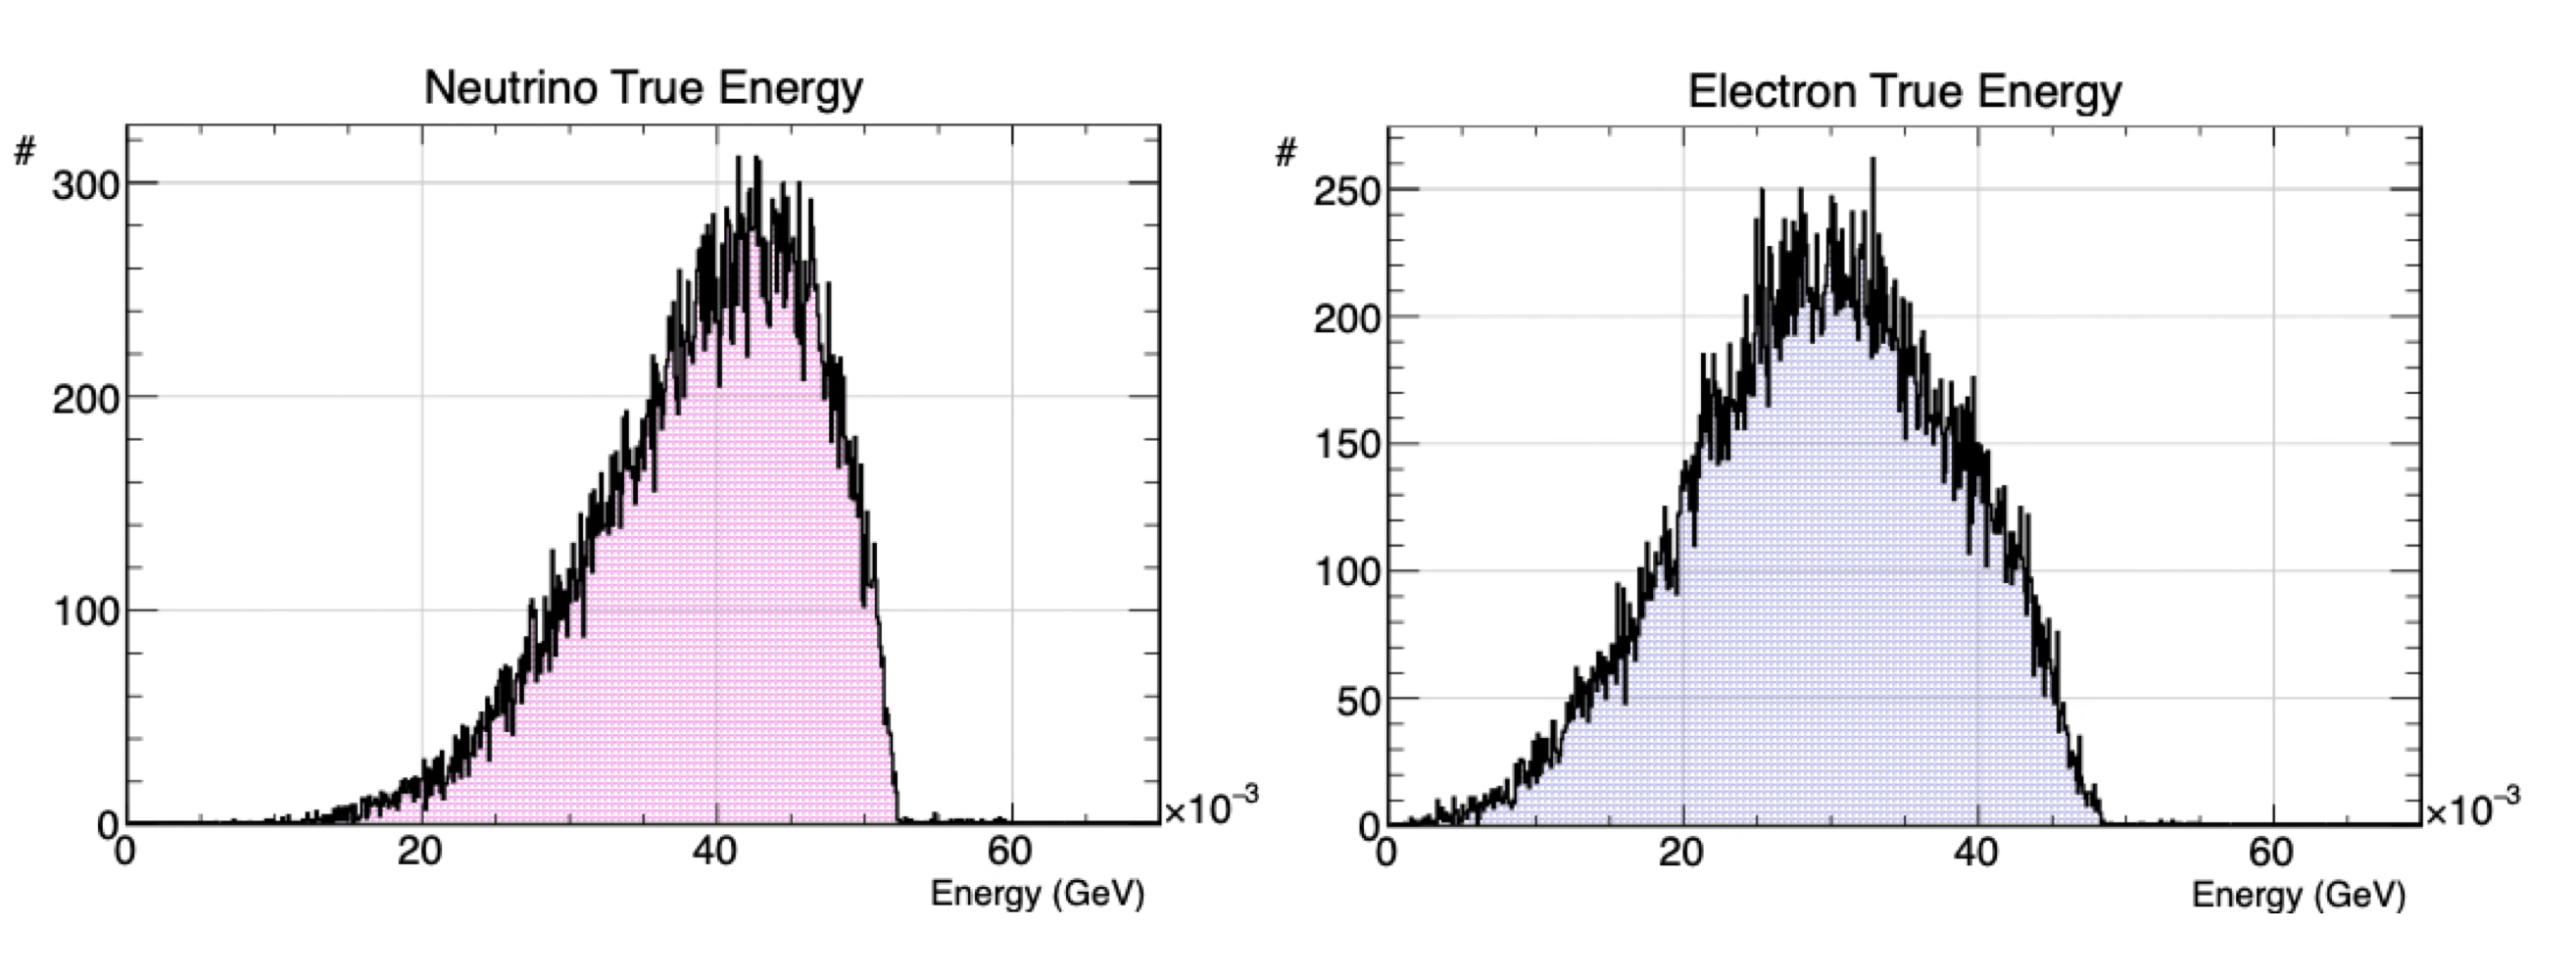
\includegraphics[width=160mm]{Figures/NuMI_muDAR_Neutrino_Electron_Energy.jpeg}
    \caption[Energy Distribution of Simulated $\mu$DAR $\nu_e$s from the NuMI Beam in MicroBooNE and the Electrons Produced in the Interaction]{{\textbf{Energy Distribution of Simulated $\mu$DAR $\nu_e$s from the NuMI Beam in MicroBooNE and the Electrons Produced in the Interaction}}\\}
    \label{sim_energy_dist_figures}
\end{figure}

\begin{figure}[h!]
    \centering
    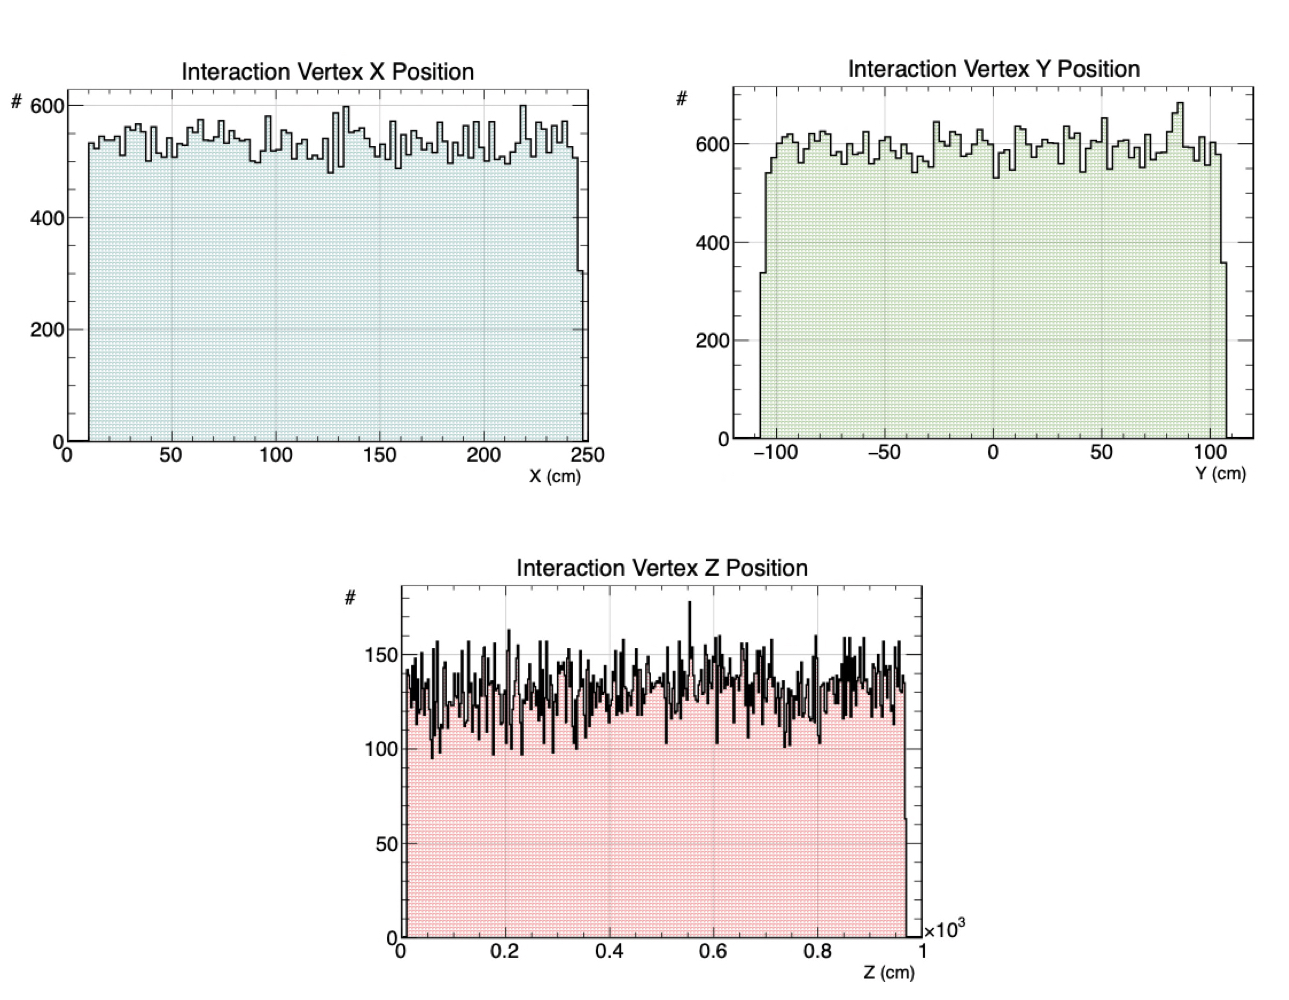
\includegraphics[width=160mm]{Figures/NuMI_muDAR_vertex.jpeg}
    \caption[Interaction Vertex Distribution of Simulated NuMI $\mu$DAR $\nu_e$s using MARLEY]{{\textbf{Interaction Vertex distribution of Simulated NuMI $\mu$DAR $\nu_e$s using MARLEY}}\\ .}
    \label{sim_vertex_dist_figures}
\end{figure}

\newpage

\section{Reconstruction of $\mu$DAR Events in MicroBooNE}

To reconstruct the events in MicroBooNE, we count on a chain of reconstruction software that processes the signal, carries it through a low level event reconstruction, up to higher level event reconstruction. In MicroBooNE, all of those are done using reconstruction algorithms that are part of LArSoft. To name the chain we used for this analysis: the signal is processed through a signal noise filter, a deconvolution algorithm, a hit finding algorithm, and the blip reconstruction algorithm (that handles two steps: cluster finding and plane matching). I will go over what each of those steps do in this chapter, and how the final algorithm performs in the Monte Carlo simulation.  

\subsection{Signal Processing}

Once the detector captures the signals presented in figure \ref{uboone_digital_signal}, we need to convert this raw signal into usable information. 
Initially, the wires record any measured voltage as a function of time in the LArTPC during the readout window, which means it will include a lot of noise from various sources. Therefore, our first step is to pass the raw data through a noise filter algorithm. Deatils on it can be found on paper \cite{noise_filter}. You can see an example of the filters performance in figure \ref{noise_filter}. 

\begin{figure}[h!]
    \centering
    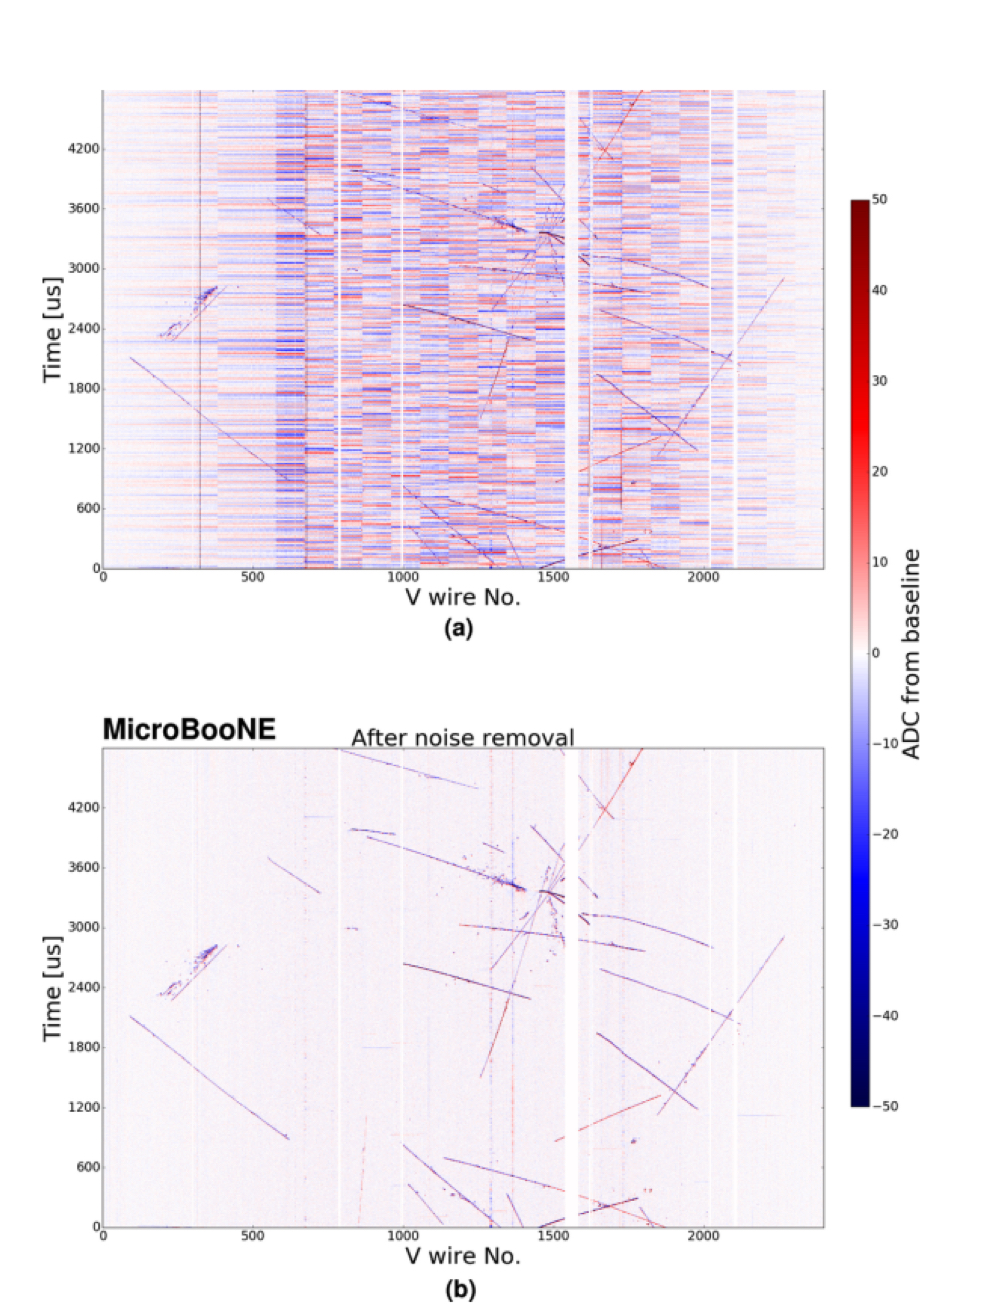
\includegraphics[width=100mm]{Figures/noise_removal.jpeg}
    \caption[MicroBooNE Software Noise Filter Performance]{{\textbf{MicroBooNE Software Noise Filter Performance}}\\ A 2D event display of the V plane from MicroBooNE data run $3493$, event $41075$ showing the raw signal (a) before and (b) after noise filtering. A clean event signature is recovered once all the identified noise sources are subtracted \cite{noise_filter}.}
    \label{noise_filter}
\end{figure}

After removing the excess noise, we need to extract the drift electron distribution from the TPC wire signals from the waveforms. The way to do this is to pass them through a 2D deconvolution procedure based on Fast Fourier Transform. This procedure suffers from low-frequency noise on the two induction planes due to the bipolar shape of the measured signals. We solve this by only considering regions of interest (ROI) on the waveforms just large enough to cover the signal. Anything that is not inside the ROI is discarded. The ROI procedure is also performed in the collection plane to reduce the data stored. The final result from this signal processing is a deconvolved wire waveform, in which a single individual element of charge signal takes the form of a Gaussian function. On figure \ref{noise_deconv} you can see the impact of each of those steps on the data. A more detailed description of MicroBooNE's signal processing is available at \cite{signal_proc}. 

\begin{figure}[h!]
    \centering
    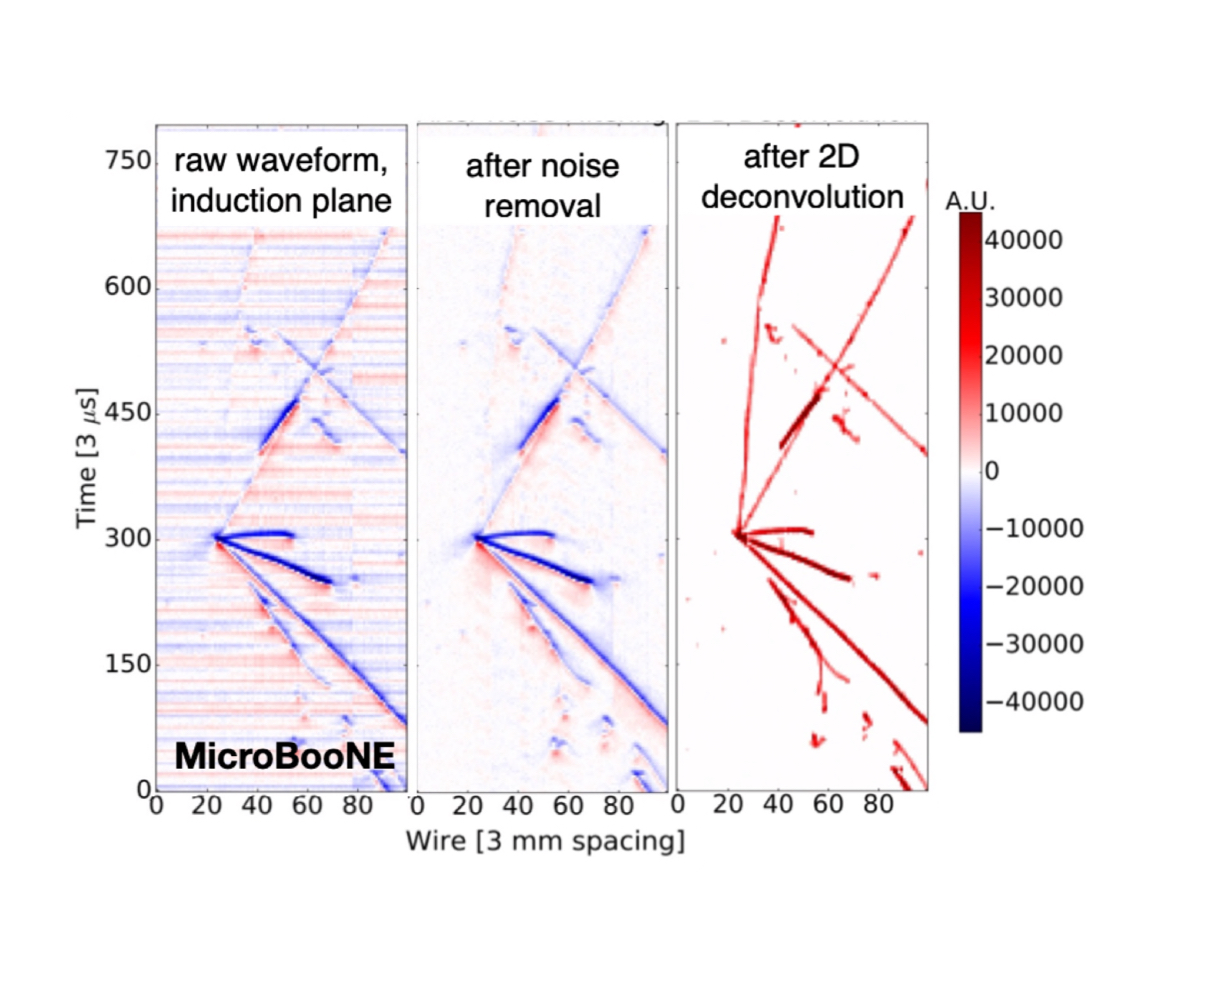
\includegraphics[width=120mm]{Figures/noise_deconv.jpeg}
    \caption[MicroBooNE Signal Processing Steps and Impact on Data]{{\textbf{MicroBooNE Signal Processing Steps and Impact on Data}}\\ 2D event displays of the U plane from MicroBooNE data run $3493$, event $41075$, zoomed in on a neutrino interaction candidate. The left-most image shows the raw digitized waveform in units of average baseline-subtracted analog-to-digital converter (ADC) scaled by $250$ per $3$ $\mu$s. The next panel shows the image after the noise removal algorithm, again in units of average baseline-subtracted ADC scaled by $250$ per $3$ $\mu$s. The last panel shows the image after processing with 2D deconvolution, also in units of electrons per $3$ $\mu$s. Adapted from \cite{Lauren_thesis}.}
    \label{noise_deconv}
\end{figure}

\subsection{Hit Finding}

The first low level reconstruction done in the signal is the ``hit finding". In it, the wire waveforms are scanned and, in case its local maxima is above a given threshold, the signal is fit into a Gaussian curve and called a ``hit". The curve's height, area, and peak time are recorded. The number of electrons detected by the wire is proportional to the area of the hit \cite{avinay_thesis}.

\subsection{Pandora}

Pandora is the multi-algorithm pattern recognition framework used by MicroBooNE to identify and reconstruct tracks in the LArTPC. It takes in the hits information in each plane and combines them to build three 2D images. Assuming the drift (x) direction is common among them, Pandora combines the different views and forms a 3D reconstruction. Beyond that, Pandora uses pattern recognition to identify the topology of the events. In a first step, Pandora tags cosmic muons and removes the associated hits. Once we have a cosmic-muons-free hit collection, Pandora works by identifying neutrino interaction vertices and reconstructing tracks and showers from it. You can see an example of a simulated neutrino interaction reconstructed using Pandora in \ref{pandora}. More information on the Pandora algorithms' use in MicroBooNE can be found in the paper \cite{pandora}.

Although Pandora is optimized to reconstruct tracks, it is not developed to identify smaller, blip-like depositions characteristic of the MeV-scale neutrino interactions. In this work, we use a combination of Pandora and Blip Reconstruction algorithms to identify the $\mu$DAR neutrino candidates. 

\begin{figure}[h!]
    \centering
    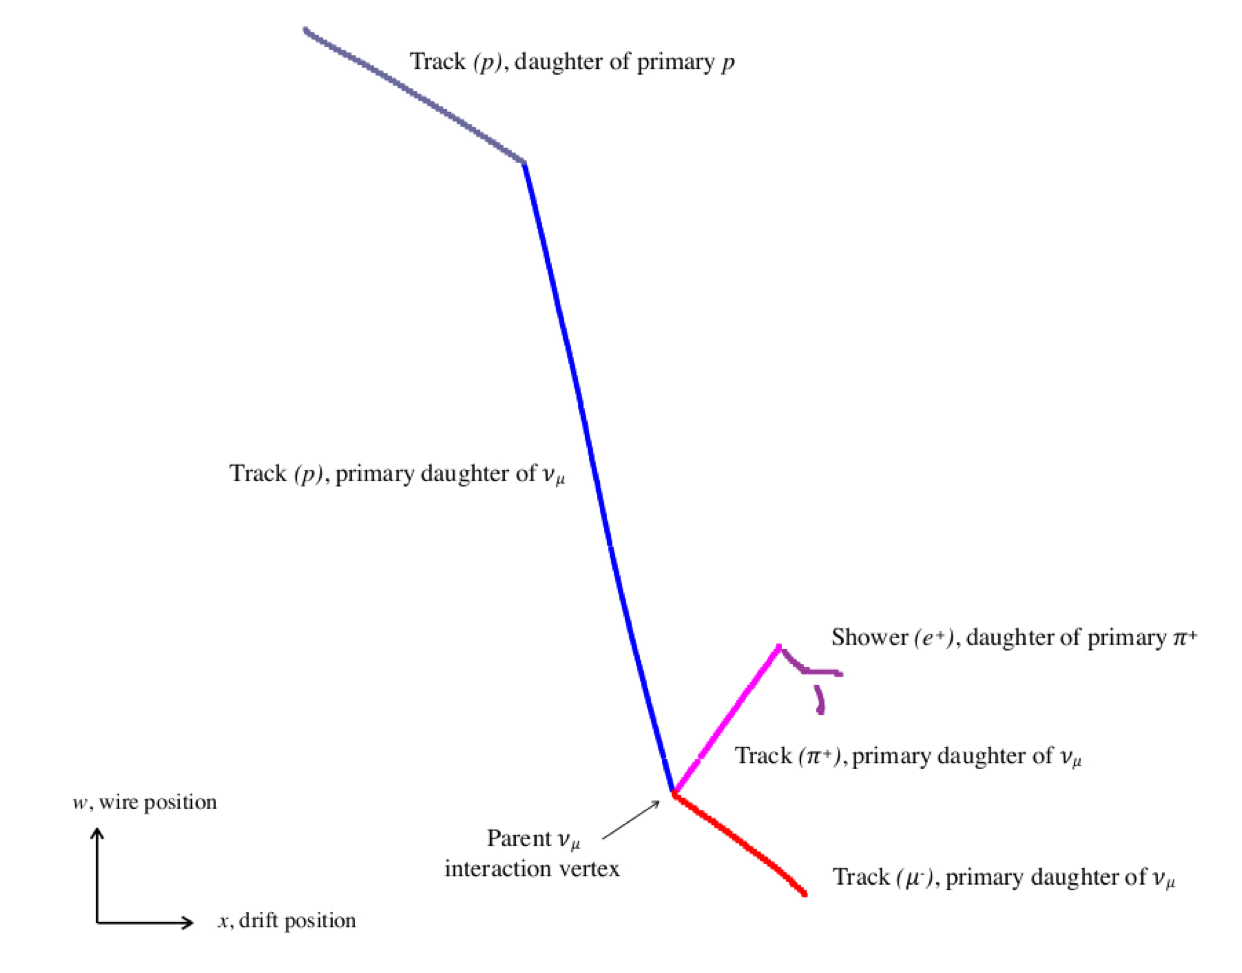
\includegraphics[width=110mm]{Figures/pandora.jpeg}
    \caption[Simulated Neutrino Interaction Reconstructed Using Pandora]{{\textbf{Simulated Neutrino Interaction Reconstructed Using Pandora}}\\ Illustration of the Pandora recontruction of a simulated charged current $\nu_{\mu}$ interaction in MicroBooNE and its products. The interaction includes a muon, proton and charged pion in the visible final state \cite{pandora}.}
    \label{pandora}
\end{figure}

\subsection{Blip Reconstruction}
The Blip Reconstruction is a class of algorithms that identifies MeV-scale charge depositions in the LArTPC and reconstruct them into 3D clusters. Those depositions, due to teir nature, resemble point-like signals, to which we call ``blips". Their reconstruction is divided in two parts: the cluster finding and the plane matching. 

On cluster finding, the algorithm works to isolate groups of hits in each of the planes. To do that, we veto 
\subsubsection{Cluster Finding}
\subsubsection{Plane Matching}


\subsubsection{$\mu$DAR events Truth versus Reco Comparitions}



\section{Data Analysis}
\subsection{Cosmic-rays Background Assessment}
\subsection{NuMI GENIE $\nu_e$ Background Assessment}
\subsection{NuMI GENIE $\nu_{\mu}$ Background Assessment}
\subsection{Data}
\section{Conclusion}